\subsection{\large{Бизнес-процессы}}
\addcontentsline{toc}{subsection}

Наиболее распространёнными вариантами использования системы являются следующие:
\begin{enumerate}
	\item Добавлен новый или изменены требования размещения к существующему элементу генерального плана.
	\item Подбор эффективных методик расчёта для конкретного набора входных данных.
\end{enumerate}

\textit{Первый вариант} использования системы порождает процесс проведения исследований и
внедрения алгоритмической методики.
Ниже представлена EPC-диаграмма этого процесса(см. рисунок \ \ref{pic:analysis__usecases-epc}).

Главным инициатором исследований является заказчик. Именно заказчик знает, где найти людей,
обладающих экспертными знаниями в проектировании генеральных планов.
Заказчик так же определяет приоритет добавления
новых элементов на генплане площадного объекта, а также набор требований к их размещению.

Сначала заказчик решает, требуется ли ему улучшить качество размещения уже существующего элемента
или добавить на генплан новый элемент. Затем заказчик сообщает аналитику контактную
информацию технического эксперта. Технический эксперт предоставляет презентативные данные аналитику для отладки методики,
способной удовлетворить требованиям заказчика.

После получения данных от технического эксперта аналитик оформляет их в виде доступном для загрузки в расчётный модуль.
После того как данные загружены в расчётный модуль, исследователи могут приступать к выработке решения
правильного размещения заданного объекта.

У исследователя всегда есть два варианта решения поставленной задачи: создать новую методику решения
или использовать уже существующую.
После того как сделан выбор, проводится ряд экспериментов,
наиболее удачные результаты экспериментов сохраняются и отправляются на рассмотрение аналитику.

\begin{figure}[H]
	\hspace*{2 cm}
	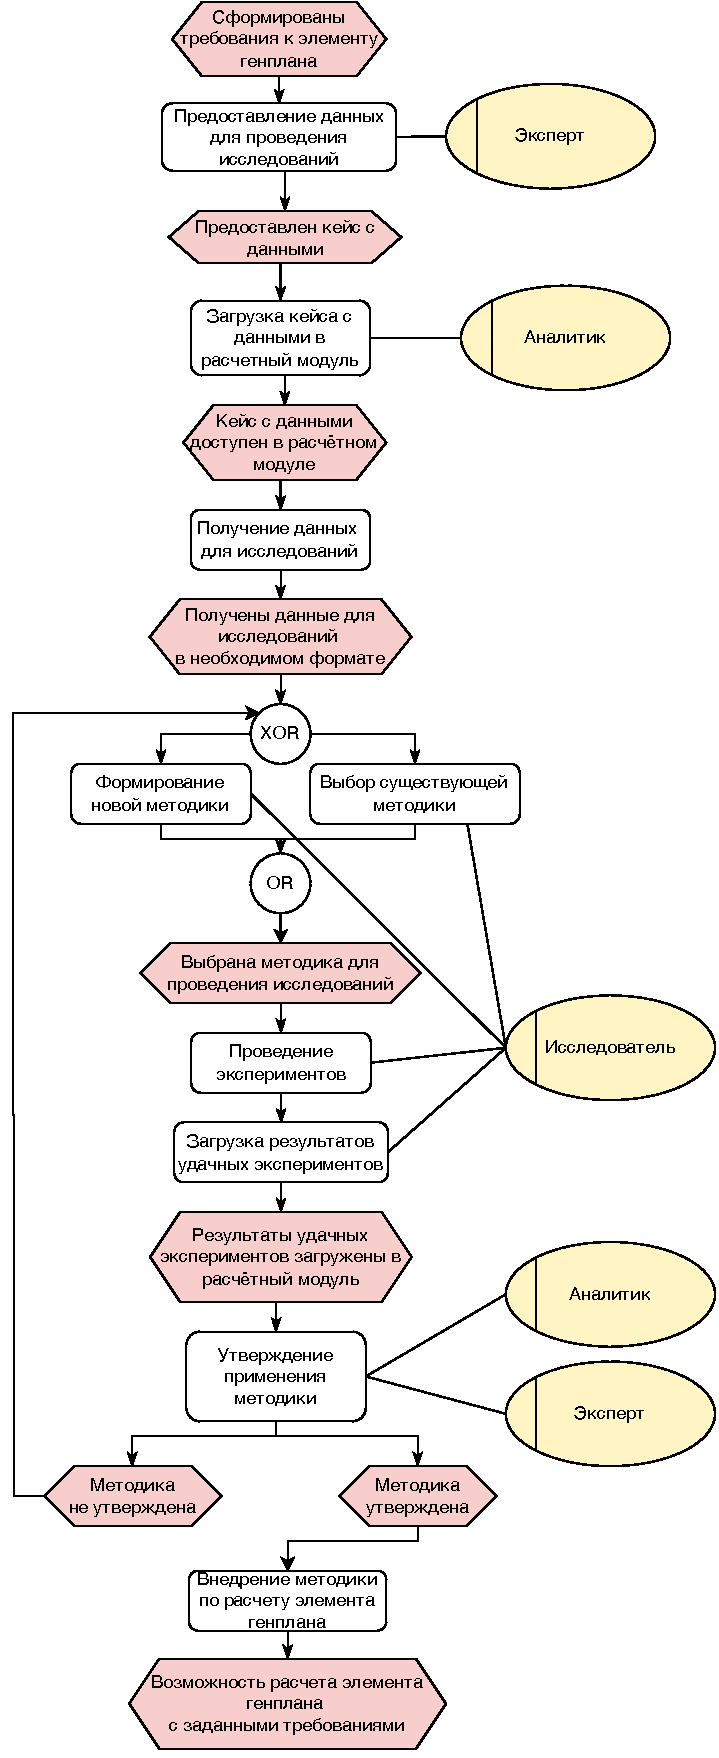
\includegraphics[width=0.64\textwidth, left]{analysis/pictures/usecases/common_epc}
	\caption{Диаграмма процесса внедрения алгоритмической методики}
	\label{pic:analysis__usecases-epc}
\end{figure}

Если аналитик делает вывод, что данная методика, позволяет получить решение, соответствующее требованиям
заказчика, то результаты эксперимента уже демонстрируются техническому эксперту со стороны заказчика,
чтобы он дополнительно убедился, что реализация данной методики не противоречит другим требованиям
проектирования генпланов.

Если замечаний к результату нет, то методика встраивается в существующее решение.
Если же есть какие-либо недостатки, то они фиксируются и устраняются.


\textit{Второй вариант} использования системы порождает бизнес-процесс
выбора наиболее эффективных методик расчёта для конкретного набора входных данных.
Он изображен на EPC-диаграмме(см. рисунок \ \ref{pic:analysis__usecases-analytics-epc}).

Все действия изображенные на этой диаграмме выполняются аналитиком в системе автоматического
расчёта генерального плана площадного объекта.
Входные данные задачи определены, на них происходит проведение анализа.
Аналитик выбирает необходимые этапы задачи и методы для проведения исследований, производит расчёты,
анализирует получившееся решение. На основании определенных критериев аналитик выбирает наиболее
эффективный набор методик для определенного набора входных данных.

\begin{figure}[H]
	\hspace*{-4.5 cm}
	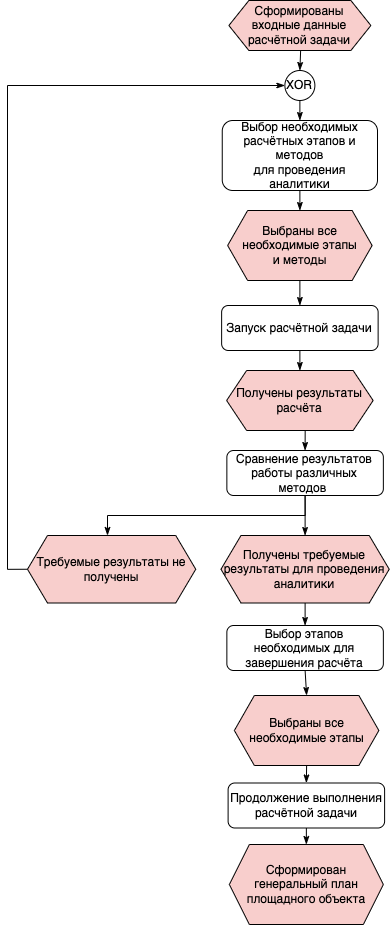
\includegraphics[width=0.64\textwidth, left]{analysis/pictures/usecases/analytics_epc}
	\caption{Диаграмма процесса выбора эффективной методики расчёта}
	\label{pic:analysis__usecases-analytics-epc}
\end{figure}
\vskip 5 mm
